%% Standalone lecture -- build with:  pdflatex -shell-escape overfitting
%% Shared preamble for standalone lecture files.
%%
%% Every lecture begins with %% Shared preamble for standalone lecture files.
%%
%% Every lecture begins with %% Shared preamble for standalone lecture files.
%%
%% Every lecture begins with \input{preamble} and is compiled on its own:
%%     pdflatex -shell-escape <lecture>
%% There is no master lectures.tex any more -- the list of lectures lives in
%% lectures.yaml and is read by the build scripts.

\documentclass[25pt,landscape,footrule]{foils}
\input{macros_gen}
\backgroundsetup{contents={}}

\usepackage{stmaryrd}
\usepackage{ifthen}
\usepackage{pdf14}

% Every figure lives in this course's lectures/figures (consolidated
% 2026-10-08).  Do not add other courses' folders back: when a name exists in
% several folders LaTeX silently takes the first, which mixed old and new
% frames of the same animation.  A missing figure should be a build error.
\graphicspath{{figures/}{../lectures/figures/}}

\date{}

\newcounter{lessoncnt}
\newcommand{\lesson}[1]{\setcounter{page}{1}%
\section{Mathematics of Machine Learning\\%
\vfill
\textcolor{red}{\textit{#1}}
\vfill}}
 and is compiled on its own:
%%     pdflatex -shell-escape <lecture>
%% There is no master lectures.tex any more -- the list of lectures lives in
%% lectures.yaml and is read by the build scripts.

\documentclass[25pt,landscape,footrule]{foils}
%\usepackage[compat2,pdftex]{geometry}
\usepackage[pdftex]{geometry}
\geometry{headsep=-2.5ex,hscale=0.9,bmargin=2.5cm,tmargin=1cm,textwidth=25cm}
\usepackage[pdftex]{xcolor}
\usepackage{pause}
\usepackage{background}
%\usepackage[color=white]{background}
\usepackage{listings}
\usepackage{graphicx}
\usepackage{epsfig}
\usepackage{epstopdf}
\usepackage{bm}
\usepackage{amssymb}
\usepackage{amsfonts}
\usepackage{marvosym}
\usepackage{cite}
\usepackage{pifont}
\usepackage[english]{babel}
\usepackage{amsmath}
\usepackage{amsfonts}
\usepackage{rotating}
\usepackage{listings}
\usepackage{pp4slide}
%\usepackage{hyperref}
\usepackage{pp4link}
\usepackage{fancyvrb}
\usepackage{multido}
\usepackage{calc}
\usepackage{mleftright}
\mleftright % Redefines \left to \mleft and \right to \mright



\thinmuskip=1mu

\newcommand{\bigstrut}{\rule[-0.5\baselineskip]{0pt}{1.2\baselineskip}}
\renewcommand{\ttdefault}{pcr}

\newcommand{\squeeze}{\setlength{\itemsep}{-2pt}}
%\renewcommand{\familydefault}{cmr}
%\renewcommand{\labelitemii}{\textcolor{green}{$\star$}}
\newcommand{\tick}{{\large \ding{51}}}
\newcommand{\cross}{{\large \ding{55}}}
%\DeclareMathAlphabet{\mat}{OT1}{cmss}{bx}{n}
\DeclareMathAlphabet{\mat}{U}{eur}{b}{n}
\newcommand{\figs}{/home/apb/figures}
\newcommand{\stimes}{{\scriptstyle \times}}
\newcommand{\tr}{\textsf{T}}
\newcommand{\e}[1]{{\rm e}^{#1}}
\newcommand{\E}[1]{{\rm e}^{{\displaystyle #1}}}
\newcommand{\av}[2][]{\mathbb{E}_{#1}\left[ #2 \right]}
\newcommand{\Var}[1]{\mathbb{V}\mathrm{ar}\left( #1 \right)}
\newcommand{\pred}[1]{\left\llbracket { \small #1} \right\rrbracket}
\newcommand{\logg}[1]{\log\left( #1 \right)}
\newcommand{\logtwo}[1]{\log_2\left( #1 \right)}
\newcommand{\bra}[1]{\left( #1 \right)}
\newcommand{\prob}[1]{\mathbb{P}\left( #1 \right)}
\newcommand{\Prob}[1]{\mathbb{P}\left( #1 \right)}
\newcommand{\Step}{\mathop{\mat{\Theta}}}
\newcommand\diag{\mathop{\mathrm{diag}}}
\newcommand{\grad}{\bm{\nabla}}
\newcommand{\gradx}{\bm{\nabla}_{\!\!\scriptscriptstyle \bm{x}}}
\newcommand{\gradw}{\bm{\nabla}_{\!\!\scriptscriptstyle \bm{w}}}
\newcommand{\dd}{\mathrm{d}}
\newcommand{\ii}{\mathrm{i}}
\newcommand{\data}{\mathcal{D}}
\newcommand{\class}{\mathcal{C}}
\newcommand{\hypo}{\mathcal{H}}
\newcommand{\indep}{\perp \!\!\!\! \perp}
\newcommand{\pd}[3][\,]{\frac{\partial^{#1}{#2}}{\partial\,{#3}}}
\newcommand{\normal}[1]{\mathcal{N}\!\left( #1 \right)}
\newcommand{\Dist}[2][Binom]{\mathrm{#1}\left( \strut {#2} \right)}
\newcommand{\brackets}[1]{\!\left( #1 \right)}
\newcommand{\KL}[2]{\mathop{\mathrm{KL}}\left(#1 \big\| #2\right)}
\newcommand{\argmax}{\mathop{\mathrm{argmax}}}
\newcommand{\argmin}{\mathop{\mathrm{argmin}}}
\newcommand{\margin}{\Delta}
\lstnewenvironment{matlab}[1][frame=TB]{\lstset{#1}}{}       
%\renewcommand{\emph}[1]{\textcolor{red}{\textbf{#1}}}
\newcommand{\myskip}[1]{}
\newcommand\mycom[2]{\genfrac{}{}{0pt}{}{#1}{#2}}
\newcommand{\jl}{\lstinline[basicstyle=\ttfamily\color{DarkGreen},%
 keywordstyle=\bfseries\ttfamily\color{DarkGreen}]}
\definecolor{EmphColor}{rgb}{0.0,0.0,1.0}
\renewcommand{\emph}[1]{{\color{EmphColor}\textbf{#1}}}
\newcommand{\len}[1]{\| #1 \|}
\newcommand{\inner}[2]{\left\langle {#1}, {#2}\right\rangle}
\newenvironment{psmallmatrix}{\left(\begin{smallmatrix}}{\end{smallmatrix}\right)}
  

\definecolor{DarkGreen}{rgb}{0,0.5,0}
\definecolor{DarkRed}{rgb}{0,0,0.5}
\definecolor{HighLight}{rgb}{1,0,0}     % yellow
\definecolor{TextColor}{rgb}{0.0,0.1,0.1}     % white
\definecolor{TwoColor}{rgb}{0.0,0.5,0.1}      % used for switching colors

\definecolor{HeadLineColor}{rgb}{1.0,0.0,0.0} % cyan
\definecolor{SpecialColor}{rgb}{0.53,0.81,1.0}
\renewcommand{\normalcolor}{\color{HeadLineColor}}

\pausecolors{TwoColor}{TextColor}{HighLight}
\pausecolors{EmphColor}{TextColor}{EmphColor}
\pausecolors{DarkGreen}{DarkGreen}{DarkRed}
\pausecolors{SpecialColor}{white}{HighLight}

\newenvironment{PauseHighLight}{\color{TwoColor}\pausehighlight}{}
\newcommand{\multipdf}[2][width=\linewidth]{\multiinclude[pause=\pauselevel{:+0}\pause,format=pdf,graphics={#1}]{#2}}

\lstdefinelanguage{pseudo}
 {keywords={all,and,begin,break,continue,do,else,elseif,%
     end,endif,endfor,endwhile,%
     exit,false,for,forall,goto,if,%
     or,return,then,true,to,repeat,until,while},%
  comment=[s]{/*}{*/},%
  morecomment=[l]//,%
  morestring=[d]"%
 }[keywords,comments,strings]


\lstloadlanguages{Java,pseudo,Python}
\lstset{
  basicstyle=\footnotesize\ttfamily\color{DarkGreen},
  keywordstyle=\bfseries\footnotesize\ttfamily\color{DarkGreen},
  commentstyle=\footnotesize\it\rmfamily\color{blue},
  language=Java,
  showstringspaces=false
  }


\lstnewenvironment{pseudo}[1][]{\lstset{language=pseudo,mathescape,literate={:=}{{$\gets$}}2 {!}{{$\neg$}}1 {!=}{{\!\!$\neq$\,\,}}2 {<=}{{\!\!$\leq$\,\,}}2 {>=}{{\!\!$\geq$\,\,}}2,escapechar=\#,#1}}{}
\lstnewenvironment{java}[1][]{\lstset{escapechar=\$,#1}}{}
% Python code: the language setting makes # comments use commentstyle.
% Comments stay monospaced: the default italic roman letter-spaces badly
% on listings' fixed columns.
\lstnewenvironment{python}[1][frame=TB]{\lstset{language=Python,
    commentstyle=\footnotesize\ttfamily\color{blue},#1}}{}

\MyLogo{}
%\Restriction{}
%\rightfooter{\hyperlink{overview}{$\square$}}

\newcommand{\keywords}[1]{\vfill{\noindent\it #1}}

\newcounter{outlineitem}
\setcounter{outlineitem}{0}
\newcommand{\outlineitem}[2]{\item%
  \def\targ{\value{emumi}}%
  \ifnum\value{enumi}=\value{outlineitem}%
  \color{HighLight}\textbf{#1}\toptarget{#2}\color{TextColor}%
   \else\toplink{#2}{#1}\fi
}
\color{TwoColor}


%-- Instead of writing \section we want the file structured by \section.
\newcommand{\section}[2][0]{\foilhead[#1cm]{#2}}

%-- Write each page into a \begin{slide} -- \end{slide} environment.
\newenvironment{slide}{}{\pauselevel{=1}}

\MyLogo{\pauselevel{=1}\Acrobatmenu{GoBack}{%
  \color{TextColor}{Adam Pr\"ugel-Bennett}} \hspace{2cm}
  % Clicking on the name steps one slide back.
  \toplink{firstoutline}{\color{red}Mathematics of Machine
    Learning}%
  \hspace{2cm}
  \texttt{//ecs-vlc.github.io/aice3001/}
  %Clicking on the date jumps to the last page, which should be the
  %table of contents.
  \rightfooter{\Acrobatmenu{LastPage}{\qquad%
  \textsf{\color{TextColor}\tiny\thepage}}}% page number
  % Clicking on the page number steps one slide back.
}
\raggedright
\newcommand{\Outline}{}

\newcommand{\pb}{\pausebuild \color{TwoColor}}
\newcommand{\pauseb}{\pauselevel{build, highlight}\pause}
\newcommand{\hl}[1]{\pauselevel{=1, highlight =1 :1, highlight =#1 :#1}\pause}
\newcommand{\hll}{\pauselevel{=1, highlight =1 :1}\pause}
\newcommand{\pauseh}{\pauselevel{highlight}\pause}
\newcommand{\nhl}[1]{\textcolor{TextColor}{#1}}
\newcommand{\mypl}[1]{\pauselevel{=#1 :#1}\pause}
\input supp-pdf.tex
\DeclareGraphicsRule{*}{mps}{*}{}
\usepackage{mpmulti}
%\leftheader{}
\rightheader{} % no more page numbers on top right


\hypersetup{pdftitle={ECS Lectures},pdfsubject={Machine Learning}
pdfauthor={Adam Prugel-Bennett},pdfkeywords={machine learning},
pdfpagemode={FullScreen},
bookmarksopen=false,
hypertexnames=false,pdfstartview={FitV},colorlinks,linkcolor={blue},
citecolor={green},urlcolor={blue}}



\newcommand\bluepage{
\clearpage
\renewcommand\normalcolor{\color{yellow}}
\pagecolor{blue}
\renewcommand\Black{\color{white}}
\color{white}
\hypersetup{colorlinks=true}
}

\newcommand\whitepage{
\clearpage
\renewcommand\normalcolor{\color{black}}
\pagecolor{white}
\renewcommand\Black{\color{black}}
\color{black}
\hypersetup{colorlinks=true}
}

\whitepage
\setlength{\unitlength}{1mm}

\newenvironment{leftImage}[2][0.3]{%
\begin{minipage}{#1\linewidth}
  \includegraphics[width=\linewidth]{#2}
\end{minipage}\hfill
\begin{minipage}{0.92\linewidth - #1\linewidth}}%
{\end{minipage}}

\newenvironment{rightImage}[2][0.3]{%
\newcommand{\foot}{\begin{minipage}{#1\linewidth}\includegraphics[width=0.98\linewidth]{#2}\end{minipage}}%
\begin{minipage}{0.95\linewidth - #1\linewidth}\raggedright }{\end{minipage}\hfill\foot}


%%% Local Variables: 
%%% mode: latex
%%% TeX-master: t
%%% End: 

\backgroundsetup{contents={}}

\usepackage{stmaryrd}
\usepackage{ifthen}
\usepackage{pdf14}

% Every figure lives in this course's lectures/figures (consolidated
% 2026-10-08).  Do not add other courses' folders back: when a name exists in
% several folders LaTeX silently takes the first, which mixed old and new
% frames of the same animation.  A missing figure should be a build error.
\graphicspath{{figures/}{../lectures/figures/}}

\date{}

\newcounter{lessoncnt}
\newcommand{\lesson}[1]{\setcounter{page}{1}%
\section{Mathematics of Machine Learning\\%
\vfill
\textcolor{red}{\textit{#1}}
\vfill}}
 and is compiled on its own:
%%     pdflatex -shell-escape <lecture>
%% There is no master lectures.tex any more -- the list of lectures lives in
%% lectures.yaml and is read by the build scripts.

\documentclass[25pt,landscape,footrule]{foils}
%\usepackage[compat2,pdftex]{geometry}
\usepackage[pdftex]{geometry}
\geometry{headsep=-2.5ex,hscale=0.9,bmargin=2.5cm,tmargin=1cm,textwidth=25cm}
\usepackage[pdftex]{xcolor}
\usepackage{pause}
\usepackage{background}
%\usepackage[color=white]{background}
\usepackage{listings}
\usepackage{graphicx}
\usepackage{epsfig}
\usepackage{epstopdf}
\usepackage{bm}
\usepackage{amssymb}
\usepackage{amsfonts}
\usepackage{marvosym}
\usepackage{cite}
\usepackage{pifont}
\usepackage[english]{babel}
\usepackage{amsmath}
\usepackage{amsfonts}
\usepackage{rotating}
\usepackage{listings}
\usepackage{pp4slide}
%\usepackage{hyperref}
\usepackage{pp4link}
\usepackage{fancyvrb}
\usepackage{multido}
\usepackage{calc}
\usepackage{mleftright}
\mleftright % Redefines \left to \mleft and \right to \mright



\thinmuskip=1mu

\newcommand{\bigstrut}{\rule[-0.5\baselineskip]{0pt}{1.2\baselineskip}}
\renewcommand{\ttdefault}{pcr}

\newcommand{\squeeze}{\setlength{\itemsep}{-2pt}}
%\renewcommand{\familydefault}{cmr}
%\renewcommand{\labelitemii}{\textcolor{green}{$\star$}}
\newcommand{\tick}{{\large \ding{51}}}
\newcommand{\cross}{{\large \ding{55}}}
%\DeclareMathAlphabet{\mat}{OT1}{cmss}{bx}{n}
\DeclareMathAlphabet{\mat}{U}{eur}{b}{n}
\newcommand{\figs}{/home/apb/figures}
\newcommand{\stimes}{{\scriptstyle \times}}
\newcommand{\tr}{\textsf{T}}
\newcommand{\e}[1]{{\rm e}^{#1}}
\newcommand{\E}[1]{{\rm e}^{{\displaystyle #1}}}
\newcommand{\av}[2][]{\mathbb{E}_{#1}\left[ #2 \right]}
\newcommand{\Var}[1]{\mathbb{V}\mathrm{ar}\left( #1 \right)}
\newcommand{\pred}[1]{\left\llbracket { \small #1} \right\rrbracket}
\newcommand{\logg}[1]{\log\left( #1 \right)}
\newcommand{\logtwo}[1]{\log_2\left( #1 \right)}
\newcommand{\bra}[1]{\left( #1 \right)}
\newcommand{\prob}[1]{\mathbb{P}\left( #1 \right)}
\newcommand{\Prob}[1]{\mathbb{P}\left( #1 \right)}
\newcommand{\Step}{\mathop{\mat{\Theta}}}
\newcommand\diag{\mathop{\mathrm{diag}}}
\newcommand{\grad}{\bm{\nabla}}
\newcommand{\gradx}{\bm{\nabla}_{\!\!\scriptscriptstyle \bm{x}}}
\newcommand{\gradw}{\bm{\nabla}_{\!\!\scriptscriptstyle \bm{w}}}
\newcommand{\dd}{\mathrm{d}}
\newcommand{\ii}{\mathrm{i}}
\newcommand{\data}{\mathcal{D}}
\newcommand{\class}{\mathcal{C}}
\newcommand{\hypo}{\mathcal{H}}
\newcommand{\indep}{\perp \!\!\!\! \perp}
\newcommand{\pd}[3][\,]{\frac{\partial^{#1}{#2}}{\partial\,{#3}}}
\newcommand{\normal}[1]{\mathcal{N}\!\left( #1 \right)}
\newcommand{\Dist}[2][Binom]{\mathrm{#1}\left( \strut {#2} \right)}
\newcommand{\brackets}[1]{\!\left( #1 \right)}
\newcommand{\KL}[2]{\mathop{\mathrm{KL}}\left(#1 \big\| #2\right)}
\newcommand{\argmax}{\mathop{\mathrm{argmax}}}
\newcommand{\argmin}{\mathop{\mathrm{argmin}}}
\newcommand{\margin}{\Delta}
\lstnewenvironment{matlab}[1][frame=TB]{\lstset{#1}}{}       
%\renewcommand{\emph}[1]{\textcolor{red}{\textbf{#1}}}
\newcommand{\myskip}[1]{}
\newcommand\mycom[2]{\genfrac{}{}{0pt}{}{#1}{#2}}
\newcommand{\jl}{\lstinline[basicstyle=\ttfamily\color{DarkGreen},%
 keywordstyle=\bfseries\ttfamily\color{DarkGreen}]}
\definecolor{EmphColor}{rgb}{0.0,0.0,1.0}
\renewcommand{\emph}[1]{{\color{EmphColor}\textbf{#1}}}
\newcommand{\len}[1]{\| #1 \|}
\newcommand{\inner}[2]{\left\langle {#1}, {#2}\right\rangle}
\newenvironment{psmallmatrix}{\left(\begin{smallmatrix}}{\end{smallmatrix}\right)}
  

\definecolor{DarkGreen}{rgb}{0,0.5,0}
\definecolor{DarkRed}{rgb}{0,0,0.5}
\definecolor{HighLight}{rgb}{1,0,0}     % yellow
\definecolor{TextColor}{rgb}{0.0,0.1,0.1}     % white
\definecolor{TwoColor}{rgb}{0.0,0.5,0.1}      % used for switching colors

\definecolor{HeadLineColor}{rgb}{1.0,0.0,0.0} % cyan
\definecolor{SpecialColor}{rgb}{0.53,0.81,1.0}
\renewcommand{\normalcolor}{\color{HeadLineColor}}

\pausecolors{TwoColor}{TextColor}{HighLight}
\pausecolors{EmphColor}{TextColor}{EmphColor}
\pausecolors{DarkGreen}{DarkGreen}{DarkRed}
\pausecolors{SpecialColor}{white}{HighLight}

\newenvironment{PauseHighLight}{\color{TwoColor}\pausehighlight}{}
\newcommand{\multipdf}[2][width=\linewidth]{\multiinclude[pause=\pauselevel{:+0}\pause,format=pdf,graphics={#1}]{#2}}

\lstdefinelanguage{pseudo}
 {keywords={all,and,begin,break,continue,do,else,elseif,%
     end,endif,endfor,endwhile,%
     exit,false,for,forall,goto,if,%
     or,return,then,true,to,repeat,until,while},%
  comment=[s]{/*}{*/},%
  morecomment=[l]//,%
  morestring=[d]"%
 }[keywords,comments,strings]


\lstloadlanguages{Java,pseudo,Python}
\lstset{
  basicstyle=\footnotesize\ttfamily\color{DarkGreen},
  keywordstyle=\bfseries\footnotesize\ttfamily\color{DarkGreen},
  commentstyle=\footnotesize\it\rmfamily\color{blue},
  language=Java,
  showstringspaces=false
  }


\lstnewenvironment{pseudo}[1][]{\lstset{language=pseudo,mathescape,literate={:=}{{$\gets$}}2 {!}{{$\neg$}}1 {!=}{{\!\!$\neq$\,\,}}2 {<=}{{\!\!$\leq$\,\,}}2 {>=}{{\!\!$\geq$\,\,}}2,escapechar=\#,#1}}{}
\lstnewenvironment{java}[1][]{\lstset{escapechar=\$,#1}}{}
% Python code: the language setting makes # comments use commentstyle.
% Comments stay monospaced: the default italic roman letter-spaces badly
% on listings' fixed columns.
\lstnewenvironment{python}[1][frame=TB]{\lstset{language=Python,
    commentstyle=\footnotesize\ttfamily\color{blue},#1}}{}

\MyLogo{}
%\Restriction{}
%\rightfooter{\hyperlink{overview}{$\square$}}

\newcommand{\keywords}[1]{\vfill{\noindent\it #1}}

\newcounter{outlineitem}
\setcounter{outlineitem}{0}
\newcommand{\outlineitem}[2]{\item%
  \def\targ{\value{emumi}}%
  \ifnum\value{enumi}=\value{outlineitem}%
  \color{HighLight}\textbf{#1}\toptarget{#2}\color{TextColor}%
   \else\toplink{#2}{#1}\fi
}
\color{TwoColor}


%-- Instead of writing \section we want the file structured by \section.
\newcommand{\section}[2][0]{\foilhead[#1cm]{#2}}

%-- Write each page into a \begin{slide} -- \end{slide} environment.
\newenvironment{slide}{}{\pauselevel{=1}}

\MyLogo{\pauselevel{=1}\Acrobatmenu{GoBack}{%
  \color{TextColor}{Adam Pr\"ugel-Bennett}} \hspace{2cm}
  % Clicking on the name steps one slide back.
  \toplink{firstoutline}{\color{red}Mathematics of Machine
    Learning}%
  \hspace{2cm}
  \texttt{//ecs-vlc.github.io/aice3001/}
  %Clicking on the date jumps to the last page, which should be the
  %table of contents.
  \rightfooter{\Acrobatmenu{LastPage}{\qquad%
  \textsf{\color{TextColor}\tiny\thepage}}}% page number
  % Clicking on the page number steps one slide back.
}
\raggedright
\newcommand{\Outline}{}

\newcommand{\pb}{\pausebuild \color{TwoColor}}
\newcommand{\pauseb}{\pauselevel{build, highlight}\pause}
\newcommand{\hl}[1]{\pauselevel{=1, highlight =1 :1, highlight =#1 :#1}\pause}
\newcommand{\hll}{\pauselevel{=1, highlight =1 :1}\pause}
\newcommand{\pauseh}{\pauselevel{highlight}\pause}
\newcommand{\nhl}[1]{\textcolor{TextColor}{#1}}
\newcommand{\mypl}[1]{\pauselevel{=#1 :#1}\pause}
\input supp-pdf.tex
\DeclareGraphicsRule{*}{mps}{*}{}
\usepackage{mpmulti}
%\leftheader{}
\rightheader{} % no more page numbers on top right


\hypersetup{pdftitle={ECS Lectures},pdfsubject={Machine Learning}
pdfauthor={Adam Prugel-Bennett},pdfkeywords={machine learning},
pdfpagemode={FullScreen},
bookmarksopen=false,
hypertexnames=false,pdfstartview={FitV},colorlinks,linkcolor={blue},
citecolor={green},urlcolor={blue}}



\newcommand\bluepage{
\clearpage
\renewcommand\normalcolor{\color{yellow}}
\pagecolor{blue}
\renewcommand\Black{\color{white}}
\color{white}
\hypersetup{colorlinks=true}
}

\newcommand\whitepage{
\clearpage
\renewcommand\normalcolor{\color{black}}
\pagecolor{white}
\renewcommand\Black{\color{black}}
\color{black}
\hypersetup{colorlinks=true}
}

\whitepage
\setlength{\unitlength}{1mm}

\newenvironment{leftImage}[2][0.3]{%
\begin{minipage}{#1\linewidth}
  \includegraphics[width=\linewidth]{#2}
\end{minipage}\hfill
\begin{minipage}{0.92\linewidth - #1\linewidth}}%
{\end{minipage}}

\newenvironment{rightImage}[2][0.3]{%
\newcommand{\foot}{\begin{minipage}{#1\linewidth}\includegraphics[width=0.98\linewidth]{#2}\end{minipage}}%
\begin{minipage}{0.95\linewidth - #1\linewidth}\raggedright }{\end{minipage}\hfill\foot}


%%% Local Variables: 
%%% mode: latex
%%% TeX-master: t
%%% End: 

\backgroundsetup{contents={}}

\usepackage{stmaryrd}
\usepackage{ifthen}
\usepackage{pdf14}

% Every figure lives in this course's lectures/figures (consolidated
% 2026-10-08).  Do not add other courses' folders back: when a name exists in
% several folders LaTeX silently takes the first, which mixed old and new
% frames of the same animation.  A missing figure should be a build error.
\graphicspath{{figures/}{../lectures/figures/}}

\date{}

\newcounter{lessoncnt}
\newcommand{\lesson}[1]{\setcounter{page}{1}%
\section{Mathematics of Machine Learning\\%
\vfill
\textcolor{red}{\textit{#1}}
\vfill}}


\begin{document}

\lesson{Over-Fitting}
\vspace{-1cm}
\begin{center}
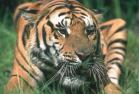
\includegraphics[width=0.45\linewidth]{tiger6} \hfill
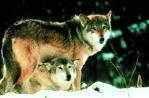
\includegraphics[width=0.45\linewidth]{wolf6}
\end{center}
\keywords{Overfitting, regularisation, feature selection}
%%%%%%%%%%%%%%%%%%%%%%% Next Slide %%%%%%%%%%%%%%%%%%%%%%%
\renewcommand{\Outline}{%
\begin{slide}
\section[1]{Outline}

\begin{minipage}{12cm}\raggedright
  \begin{enumerate}\squeeze
    \outlineitem{Over-fitting?}{overfitting}
    \outlineitem{Controlling Complexity}{complexity}
    \outlineitem{Hidden structure}{hidden}
    \outlineitem{Regularisation}{regularisers}
    \outlineitem{Double Descent}{doubledescent}
  \end{enumerate}
\end{minipage}\hfill
\begin{minipage}{10cm}
  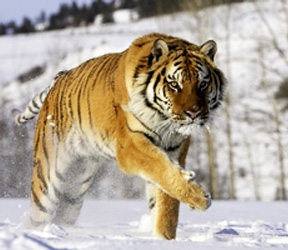
\includegraphics[width=10cm]{tiger1.jpg}
\end{minipage}
\end{slide}
\addtocounter{outlineitem}{1}
}

\setcounter{outlineitem}{1}

%%%%%%%%%%%%%%%%%%%%%%% Next Slide %%%%%%%%%%%%%%%%%%%%%%%
\Outline % Why ML works
\toptarget{firstoutline}
%%%%%%%%%%%%%%%%%%%%%%% Next Slide %%%%%%%%%%%%%%%%%%%%%%%

\begin{slide}
\section{Over-fitting}

\begin{PauseHighLight}
  \begin{itemize}
  \item Complex machines can \emph{over-fit}
    \begin{quote}
      \textit{\textbf{over-fitting}: fitting the training data well at
        the cost of getting poorer generalisation performance}\pause
    \end{quote}
  \item Three red cars\ldots\pause
  \item If we used an infinitely flexible machine we can fit our
    training data perfectly, but would have no generalisation
    ability\pause
  \end{itemize}
\end{PauseHighLight}

\end{slide}

%%%%%%%%%%%%%%%%%%%%%%% Next Slide %%%%%%%%%%%%%%%%%%%%%%%

\begin{slide}
\section[-2]{Binary Classification Task for You}

\begin{center}
  \setlength{\unitlength}{1mm}
  \begin{picture}(240,150)
    \put(115,-5){\line(0,1){145}}
    \put(114,-5){\line(0,1){145}}
    \put(116,-5){\line(0,1){145}}
    \put(0,0){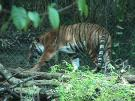
\includegraphics[width=5cm]{tiger4.png}}
    \put(60,0){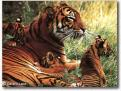
\includegraphics[width=5cm]{tiger5.png}}
    \put(0,50){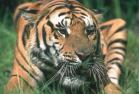
\includegraphics[width=5cm]{tiger6.png}}
    \put(60,50){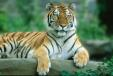
\includegraphics[width=5cm]{tiger7.png}}
    \put(0,100){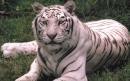
\includegraphics[width=5cm]{tiger8.png}}
    \put(60,100){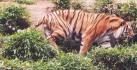
\includegraphics[width=5cm]{tiger9.png}}
    \put(120,0){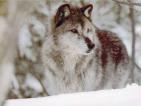
\includegraphics[width=5cm]{wolf1.png}}
    \put(180,0){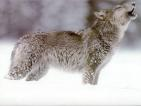
\includegraphics[width=5cm]{wolf2.png}}
    \put(120,50){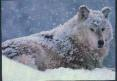
\includegraphics[width=5cm]{wolf3.png}}
    \put(180,50){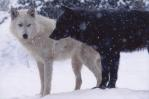
\includegraphics[width=5cm]{wolf4.png}}
    \put(120,100){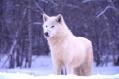
\includegraphics[width=5cm]{wolf5.png}}
    \put(180,100){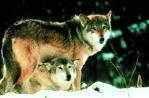
\includegraphics[width=5cm]{wolf6.png}}
    \put(55,-5){\makebox(0,0){Class 1}}
    \put(175,-5){\makebox(0,0){Class 2}}
  \end{picture}
\end{center}

\end{slide}



%%%%%%%%%%%%%%%%%%%%%%% Next Slide %%%%%%%%%%%%%%%%%%%%%%%

\begin{slide}
\section{Which Category?}

\begin{PauseHighLight}
  \begin{itemize}
  \item Which category does the following image belong to?
    \begin{center}
      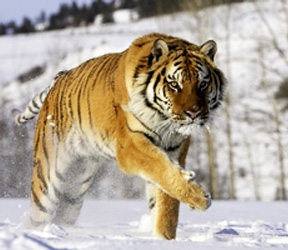
\includegraphics[height=10cm]{tiger1.jpg}
    \end{center}
  \end{itemize}
\end{PauseHighLight}

\end{slide}

%%%%%%%%%%%%%%%%%%%%%%% Next Slide %%%%%%%%%%%%%%%%%%%%%%%

\begin{slide}
\section{Spurious Rules}

\begin{PauseHighLight}
  \begin{itemize}
  \item You ask a learning machine to solve a task based on data\pause
  \item It will find a rule that does this, but not necessarily the rule
    you had in mind\pause---machine learning can't read your
    mind\pauseb
  \item Infinitely flexible machines have an infinity of spurious
    rules they can learn\pause---they are useless\pauseb
  \item What should we do?\pause
  \end{itemize}
\end{PauseHighLight}

\end{slide}

%%%%%%%%%%%%%%%%%%%%%%% Next Slide %%%%%%%%%%%%%%%%%%%%%%%

\begin{slide}
\section[-2]{All Binary Functions}

\pb \pause \pauselevel{=1}
\begin{center}
  \multipdf[width=\linewidth]{flexibleMachine}\pause
\end{center}
\end{slide}

%%%%%%%%%%%%%%%%%%%%%%% Next Slide %%%%%%%%%%%%%%%%%%%%%%%

\begin{slide}
\section{Are MLPs Universal Approximators?}
\pause
\begin{PauseHighLight}
  \begin{itemize}
  \item Yes\pauseb{} and No\pauseb
  \item Yes: If you give me any (continuous) function, I can find an MLP that
    approximates that function to any desired accuracy\pauseb{} {\small (on
    a bounded region)}\pauseb
  \item No: If you give me an MLP, I can find a function with an
    arbitrary high approximation error\pauseb
  \item Would an MLP that could approximate any function be
    useful?\pauseb
  \item \emph{Absolutely not!}\pauseb
  \end{itemize}
\end{PauseHighLight}

\end{slide}



%%%%%%%%%%%%%%%%%%%%%%% Next Slide %%%%%%%%%%%%%%%%%%%%%%%
\Outline % Controlling Complexity
%%%%%%%%%%%%%%%%%%%%%%% Next Slide %%%%%%%%%%%%%%%%%%%%%%%

\begin{slide}
\section{Controlling Complexity}

\begin{PauseHighLight}
  \begin{itemize}
  \item Infinitely flexible machines don't generalise\pause{} (because
    any unseen data could have any value)\pauseb
  \item \emph{Machine learning only works because there is
      some structure in the data}\pause
  \item A successful machine should capture this structure\pause
  \item Even deep learning machines with millions or billions of
    parameters only work because they successfully capture the
    structure of images or text\pause
  \item Different learning machines have different performance on
    different problems because the data has different structure\pause
  \end{itemize}
\end{PauseHighLight}

\end{slide}


%%%%%%%%%%%%%%%%%%%%%%% Next Slide %%%%%%%%%%%%%%%%%%%%%%%


\begin{slide}
\section{Training Examples}

\begin{PauseHighLight}
  \begin{itemize}
  \item As we increase the number of training examples, we make it harder
    to find a spurious rule\pause
  \item Bigger data sets allow us to use more complicated
    machines\pause
  \item Part of the success of deep learning is because it uses huge
    training sets\pause---but this is only a part of their success\pauseb
  \item (Labelled) data is often expensive to collect so we
    sometimes have no choice but to use a small training set\pause
  \item One of the limitations of using deep learning comes because we often
    have limited data\pause
  \end{itemize}
\end{PauseHighLight}

\end{slide}


%%%%%%%%%%%%%%%%%%%%%%% Next Slide %%%%%%%%%%%%%%%%%%%%%%%

\begin{slide}
\section{Preprocessing}

\begin{PauseHighLight}
  \begin{itemize}
  \item Structure might often be obscure to the learning machine\pause
  \item If we are trying to predict the spread of disease then a list
    of place names might be a lot less useful than their
    coordinates\pause
  \item Imposing an ordering on an unordered set might \textbf{not} be useful
    \begin{align*}
      \left\{\strut \text{``blue''}:0,\;\text{``brown''}:1,\;
      \text{``green''}:2,\;\text{``black''}:3 \right\}\pause
    \end{align*}
  \item Choosing an encoding that reflect meaningful structure is
    essential to successful machine learning\pause
  \end{itemize}
\end{PauseHighLight}

\end{slide}

%%%%%%%%%%%%%%%%%%%%%%% Next Slide %%%%%%%%%%%%%%%%%%%%%%%
\Outline % Hidden structure
%%%%%%%%%%%%%%%%%%%%%%% Next Slide %%%%%%%%%%%%%%%%%%%%%%%

\begin{slide}
  \section{Hidden Structure}

  \begin{PauseHighLight}
    \begin{itemize}
    \item Often the structure of data is invisible to us\pause
    \item A very successful strategy is to try many different machine
      learning techniques and choose the best\pause{} (stupid but
      effective)\pauseb
    \item Often learning machines have adjustable parameters
      (hyper-parameters) that we have to set (they are the same for
      all input data, but change with the problem)\pause
    \item We need to choose the hyper-parameters to fit the data in
      our problem\pause
    \item Fine tuning hyper-parameters is important\pause{} and almost always
      required (true in SVMs, MLP, deep learning)\pauseb
    \end{itemize}
  \end{PauseHighLight}

\end{slide}

%%%%%%%%%%%%%%%%%%%%%%% Next Slide %%%%%%%%%%%%%%%%%%%%%%%

\begin{slide}
\section{Measuring Generalisation Performance}

\begin{PauseHighLight}
  \begin{itemize}
  \item Recall, we want to predict \emph{unseen} data\pause
  \item \emph{You cannot use data that you have trained
      on!}\pause---you will overfit\pauseb
  \item Need to split your data up into training and validation
    set\pause
  \item Use the validation set to choose the hyper-parameters\pause
  \item You need a separate testing set if you want to measure your
    generalisation performance\pause
  \end{itemize}
\end{PauseHighLight}

\end{slide}

%%%%%%%%%%%%%%%%%%%%%%% Next Slide %%%%%%%%%%%%%%%%%%%%%%%

\begin{slide}
\section[-2]{The Overfitting Game}

\pb\pause\pauselevel{=1}
\begin{center}
  \multipdf[width=\linewidth]{overfit}\pause
\end{center}

\end{slide}



%%%%%%%%%%%%%%%%%%%%%%% Next Slide %%%%%%%%%%%%%%%%%%%%%%%

\begin{slide}
  \section[-2]{Cross Validation}
  
\pb
\begin{itemize}
\item If you want to use more data for training then you can use cross
  validation\pauseh
\item $K$-fold cross validation splits the data into $K$ groups\pauseh
\end{itemize}
\begin{center}
  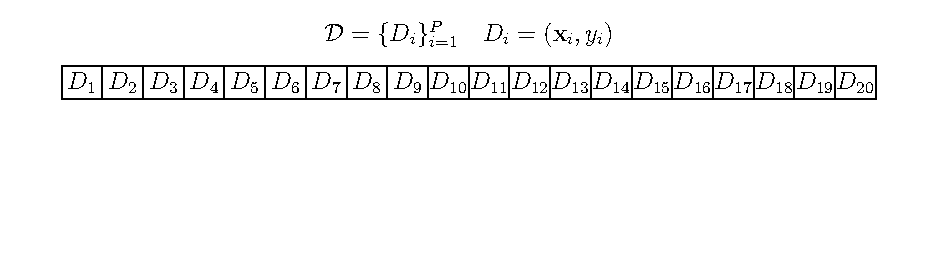
\includegraphics[width=0.9\linewidth]{cross_validation0}\mypl{1 :3}
  \multido{\ia=1+1,\ib=4+1}{23}{%
    \llap{\includegraphics[width=0.9\linewidth]{cross_validation\ia}}\mypl{\ib}}
  \llap{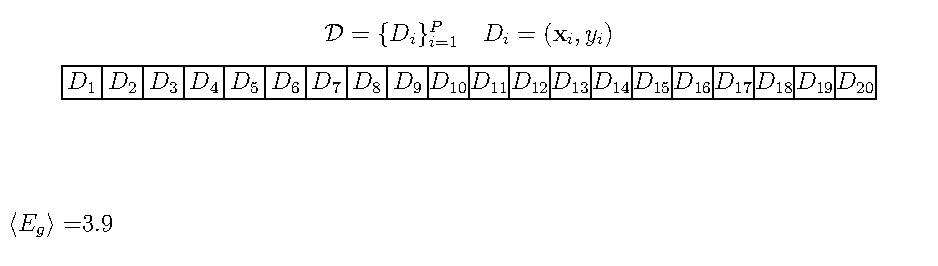
\includegraphics[width=0.9\linewidth]{cross_validation23}}
\end{center}
\begin{itemize}
\item Leave-one-out cross-validation is extreme case\pause
\end{itemize}
\end{slide}



%%%%%%%%%%%%%%%%%%%%%%% Next Slide %%%%%%%%%%%%%%%%%%%%%%%

\begin{slide}
\section[-2]{Hidden Structure}

\pb
Can't spot low dimensional data by looking at numbers\pause
\begin{center}
  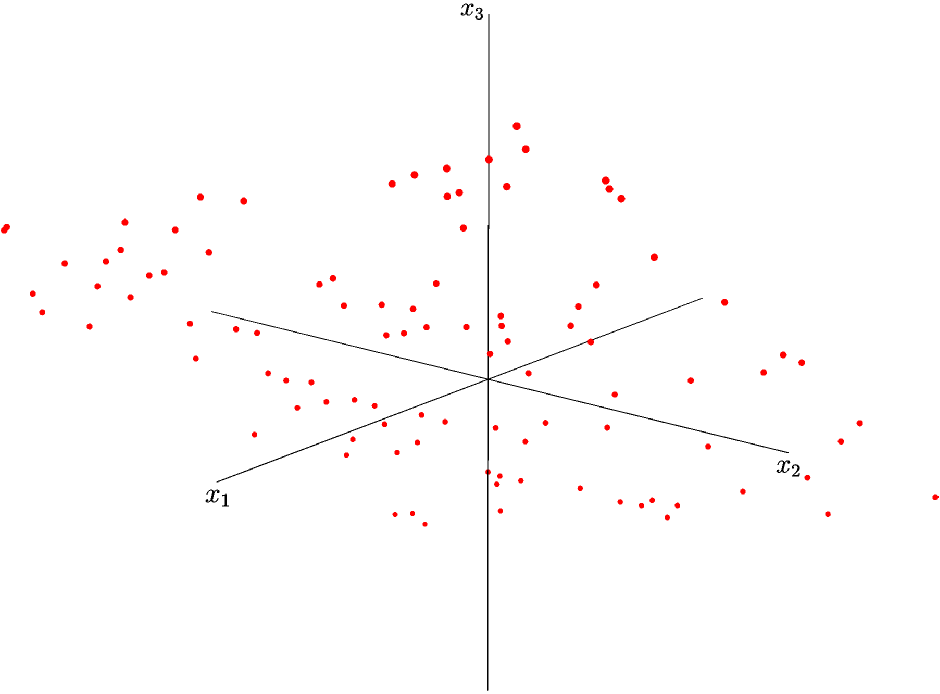
\includegraphics[width=0.7\linewidth]{rotate3d0}\mypl{1}
  \multido{\ia=1+1,\ib=2+1}{6}{%
    \llap{\includegraphics[width=0.7\linewidth]{rotate3d\ia}}\mypl{\ib}}
\end{center}

\end{slide}


%%%%%%%%%%%%%%%%%%%%%%% Next Slide %%%%%%%%%%%%%%%%%%%%%%%

\begin{slide}
\section[-1]{Feature Selection}

\begin{PauseHighLight}
  \begin{itemize}
  \item Spurious features will allow us to find spurious rules
    (\emph{over-fitting})\pause
  \item We can try different combinations of features to find the best
    set, although it rapidly becomes intractable to do this in all
    ways\pause
  \item We can use heuristics to decide which features to keep (none
    is fail-safe), or project onto a few principal components (PCA)\pause
  \item Feature selection however can be powerful, often we can get very
    good results by keeping only a few variables\pause
  \item As well as possibly improving generalisation we also get a more
    \emph{interpretable} rule\pause
  \end{itemize}
\end{PauseHighLight}

\end{slide}

%%%%%%%%%%%%%%%%%%%%%%% Next Slide %%%%%%%%%%%%%%%%%%%%%%%

\begin{slide}
\section{Normalising Features}

\begin{PauseHighLight}
  \begin{itemize}
  \item Measuring a feature in millimeters or kilometers is going
    to make a lot of difference to the size of that feature\pause
  \item Many learning algorithms are sensitive to the size of a
    feature (larger features are more important)\pause
  \item If we don't know how important different features are then it
    makes sense to normalise our features\pause, E.g.
    \begin{align*}
      x^\alpha_i &\leftarrow \frac{x^\alpha_i-\hat{\mu}_i}{\hat{\sigma}_i},
      &
      \hat{\mu}_i &= \frac{1}{m} \sum_{\beta=1}^m x_i^\beta,
      &
      \hat{\sigma}_i^2 &= \frac{1}{m-1} \sum_{\beta=1}^m
                       (x_i^\beta-\hat{\mu}_i)^2\pauseb 
    \end{align*}
  \end{itemize}
\end{PauseHighLight}

\end{slide}




%%%%%%%%%%%%%%%%%%%%%%% Next Slide %%%%%%%%%%%%%%%%%%%%%%%
\Outline % Regularisation
%%%%%%%%%%%%%%%%%%%%%%% Next Slide %%%%%%%%%%%%%%%%%%%%%%%

\begin{slide}
\section[-2]{Explicit Regularisation}

\begin{PauseHighLight}
  \begin{itemize}
  \item As in ridge regression, we can modify our error function to
    choose smoother functions
    \begin{align*}
      L = \sum_{k=1}^m \left( \bm{w}^\tr \, \bm{x}_k - y_k \right)^2\pause
      + \eta \, \|\bm{w}\|^2\pauseb
    \end{align*}
    (Good to normalise features)\pauseb
  \item Second term is minimised when $w_i=0$\pause
  \item If $w_i$ is large then
    \begin{align*}
      f(\bm{x}|\bm{w})= \bm{w}^\tr \, \bm{x}\pause = \sum_{i=1}^p
      w_i \, x_{i}\pauseb
    \end{align*}
    varies rapidly as we change $x_i$\pause    
  \end{itemize}
\end{PauseHighLight}

\end{slide}

%%%%%%%%%%%%%%%%%%%%%%% Next Slide %%%%%%%%%%%%%%%%%%%%%%%

\begin{slide}
\section[-1]{Regularisers Are Priors}

\begin{PauseHighLight}
  \begin{itemize}
  \item Recall MAP: maximise $\log f(\data|\bm{w}) + \log f(\bm{w})$, so
    $-\log f(\bm{w})$ is a regulariser\pause
  \item Gaussian noise of variance $\sigma^2$ and a Gaussian prior
    $w_i\sim\mathcal{N}(0,s^2)$ give ridge regression with
    $\eta = \sigma^2/s^2$\pause
  \item A Laplace prior $f(w_i)\propto\e{-|w_i|/b}$ gives the
    \emph{lasso} penalty $\eta\sum_i|w_i|$\pause
  \item The prior says what we believe before seeing data: small
    weights, or few non-zero weights\pause
  \item Regularisation is how we tell the machine about the structure
    we expect\pause
  \end{itemize}
\end{PauseHighLight}

\end{slide}


%%%%%%%%%%%%%%%%%%%%%%% Next Slide %%%%%%%%%%%%%%%%%%%%%%%

\begin{slide}
\section[-2.5]{Lasso}

\pb
\begin{itemize}\squeeze
\item We can use other regularisers
  \begin{align*}
    L = \sum_{k=1}^m \left( \bm{w}^\tr \, \bm{x}_k - y_k \right)^2\pauseh
    + \eta \, \sum_{i=1}^p |w_i| \pauseb
  \end{align*}
\item Spurious features (e.g. colour of flag on energy consumption) will
  give us a small improvement in training error\pauseh
  \begin{center}
    \multipdf[width=0.7\linewidth]{lasso}\pause
  \end{center}
\end{itemize}


\end{slide}

%%%%%%%%%%%%%%%%%%%%%%% Next Slide %%%%%%%%%%%%%%%%%%%%%%%

\begin{slide}
\section[-2]{Early Stopping Is Implicit Ridge}

\begin{PauseHighLight}
  \begin{itemize}\squeeze
  \item Some machines regularise without an explicit penalty\pause
  \item Gradient descent on $\frac12\|\mat{X}\bm{w}-\bm{y}\|^2$ from
    $\bm{w}=\bm{0}$ with learning rate $r$: in the SVD basis, after $t$
    steps component $k$ is
    \begin{align*}
      \Bigl(1 - (1 - r\,s_k^2)^t\Bigr) \times \text{(least squares
      component)}\pause
    \end{align*}
  \item Ridge regression multiplies the same component by
    $s_k^2/(s_k^2+\eta)$\pause
  \item Both keep the directions with large $s_k$ and suppress those with
    small $s_k$, where the variance lives\pause
  \item So stopping early acts like ridge with $\eta\approx1/(r\,t)$:
    training time is a regulariser\pause
  \end{itemize}
\end{PauseHighLight}

\end{slide}


%%%%%%%%%%%%%%%%%%%%%%% Next Slide %%%%%%%%%%%%%%%%%%%%%%%

\begin{slide}
  \section[-2]{Maximum Margin Machines}
  \pb
  \begin{itemize}
  \item Perceptrons have many options to separate data\pauseh
    \begin{center}
      \multipdf[width=0.8\linewidth]{maxMargin}\pause
    \end{center}
  \item SVMs choose the machine with the biggest margins\pause
  \end{itemize}
\end{slide}

%%%%%%%%%%%%%%%%%%%%%%% Next Slide %%%%%%%%%%%%%%%%%%%%%%%

\begin{slide}
\section[-1]{Why SVMs Generalise}

\begin{PauseHighLight}
  \begin{itemize}
  \item For data in a ball of radius $R$ separated with margin
    $\gamma$, the capacity of the machine depends on $(R/\gamma)^2$,
    not on the dimension of the feature space\pause
  \item That is why the kernel trick, with enormous (even infinite)
    feature spaces, need not over-fit\pause
  \item Removing a training point that is not a support vector leaves
    the solution unchanged, so the leave-one-out error is at most
    (number of support vectors)$/m$\pause
  \item Few support vectors and a large margin mean good
    generalisation\pause
  \item But you still need to normalise the features and tune $C$
    (and the kernel parameters)\pause
  \end{itemize}
\end{PauseHighLight}

\end{slide}


%%%%%%%%%%%%%%%%%%%%%%% Next Slide %%%%%%%%%%%%%%%%%%%%%%%

\Outline % Double Descent
%%%%%%%%%%%%%%%%%%%%%%% Next Slide %%%%%%%%%%%%%%%%%%%%%%%

\begin{slide}
\section[-2]{Double Descent}

\begin{center}
  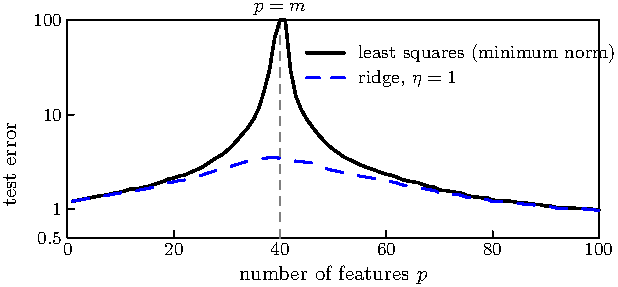
\includegraphics[width=0.85\linewidth]{doubleDescent-0}
\end{center}
\begin{PauseHighLight}
  \begin{itemize}\squeeze
  \item Least squares on $m=40$ points using $p$ of 100 features\pause
  \item The classical U-curve, a spike at $p=m$, then a second
    descent\pause
  \end{itemize}
\end{PauseHighLight}

\end{slide}

%%%%%%%%%%%%%%%%%%%%%%% Next Slide %%%%%%%%%%%%%%%%%%%%%%%

\begin{slide}
\section[-1]{Why Bigger Can Be Better}

\begin{PauseHighLight}
  \begin{itemize}
  \item At $p=m$ there is exactly one fit through every (noisy) point;
    the smallest singular value is near 0, so the variance
    $\sum_k\sigma^2/s_k^2$ explodes\pause
  \item For $p>m$ there are infinitely many exact fits; we take the one
    with the smallest $\|\bm{w}\|$\pause
  \item Gradient descent from $\bm{w}=\bm{0}$ finds exactly this
    minimum-norm solution\pause{}: an implicit regulariser\pauseb
  \item Modern networks have far more parameters than data, yet trained
    with (S)GD they often generalise well\pause
  \item Counting parameters is not the same as measuring
    complexity\pause
  \end{itemize}
\end{PauseHighLight}

\end{slide}

%%%%%%%%%%%%%%%%%%%%%%% Next Slide %%%%%%%%%%%%%%%%%%%%%%%

\begin{slide}
\section{Lessons}

\begin{PauseHighLight}
  \begin{itemize}
  \item Machine learning isn't magic\pause
  \item It works when the learning machine is well attuned to the
    problem\pause
  \item Sometimes you can help by preprocessing your data\pause
  \item Regularisers (explicit, priors, or implicit like early
    stopping and minimum norm) select simpler machines\pause
  \item Most machines have hyper-parameters that you tune to match the
    machine to the data\pause
  \item Complexity is not just the number of parameters: margins and
    norms matter\pause
  \end{itemize}
\end{PauseHighLight}

\end{slide}



%%% Local Variables:
%%% TeX-master: "lectures"
%%% End:

\end{document}
